%%%%% New Chapter %%%%%
%%%%% New Chapter %%%%%
%\newchapt{Dataset Segmentation}{chapt_segment}{Model Segmentation}
\section{Dataset Segmentation}
\label{sec:mseg}

Modeling a building PCD as a whole structure simultaneously 
is complicated due to the natural complexity of buildings.
To simplify this problem, 
We utilize the divide and conquer strategy 
to segment the whole PCD of a building into simpler ones.
Following this, we reconstruct each segmented 
part based on extrusion or tapering operations.
Once each segment is processed and modeled, 
the whole PCD can be combined and merged into the final model.

3D point cloud data segmentation has been an active research topic for years,
and Hoover {\it et al.} compared a variety of methods 
for finding planar segments in range images \cite{MS_HOO}.
Essentially, segmentation is the process of labeling each data point
so that the points belonging to the same structure are grouped together.
Based on the techniques used for segmentation, 
the proposed algorithms can be roughly categorized into two groups.

\begin{enumerate}

\item {\bf Edge based method:}

Edge based methods first apply edge detector to
extract the boundary edges of different regions.
The edges are detected based on the local surface properties, 
such as surface normals, gradients, principal curvatures, 
or higher order derivatives.
These edges include jump edges, crease edges and smooth edges \cite{MS_JBU}.
Jump edges are defined as discontinuities in depth values, 
which are observed when an object is occluded by another one.
Crease edges are characterized by discontinuities in surface normals,
which are formed where two regions meet.
Smooth edges are those with continuous surface normals but 
discontinuous curvatures.
The second stage of these methods is to link these detected edges
to form closed regions for segmentation \cite{MS_SV,MS_KS}.

The main weakness of these methods is that 
they cannot guarantee closed boundaries 
for the complicated situations where some edge points 
may not be correctly detected.
To tackle this issue, edge detection based on
scan line approximation are proposed as in\cite{MS_SD,MS_KMK,MS_JB}.
Scan-line based methods first project the range data into 
binary edge map along a given direction or scan line. 
For example, a scan line on 3D plane produces a 3D straight line.
After projection, scan line segments are merged together
based on some similarity measure in a region-growing fashion.
Finally, some edge grouping techniques, such as 
minimum spanning tree, are applied to obtain closed contours
for segmentation.
The scan line method is mainly designed to extract planar surfaces.

Heath {\it et al.} compared some well-known edge detectors,
such as Canny, Nalwa-Binford, Sarkar-Boyer and Sobel \cite{MS_HSSB}.
There are several criteria they used for comparison:
For each edge detector, 
is it possible to choose a single set of optimal parameters 
for all the images without significantly affecting the performance?
Does an edge detector produce edges of the same quality for all images
or does the edge quality vary with input images?
They found that the optimal parameter settings of an edge detector
are strongly dependent on the input images,
and that the relative performance of the edge detectors varied 
statistically significantly across the input images.
This indicates the performance of the dataset segmentation
might be affected by the parameter settings of its edge detector
and there is no optimal detector that can be used for any input data.


\item {\bf Region based method:}

The majority work on range image segmentation relied on 
region-based techniques \cite{MS_XW,MS_RHV,MS_PV}.
These methods are relatively less sensitive to the noise in the data,
and usually perform better when compared to edge-detection methods.
First, seed regions which can be planar or non-planar 
surface patches are computed.
Least squares adjustment and Hough transform are robust methods 
to detect planar seeds.
The seed regions are then gradually growing to larger region 
by grouping points around them based on the given similarity measure, 
such as slope, curvature or surface normal. 

Region based approaches are essentially focusing on local features
and their consistencies in the data.
For example, Hernandez {\it et al.} extracted features from connected components
based on Top-Hat of hole filling algorithm of range images \cite{MS_HMP}.
Although these techniques bring acceptable results, 
they suffered from some common issues, 
such as the selection of the initial seed regions
and the determination of the number of clusters.
Some global features based on graph techniques are proposed to improve
segmentation results.
Graph cut in \cite{MS_SM,MS_BK} and minimum spanning tree in \cite{MS_HK}
are widely used graph based algorithms.
The observation is that data points in the same segment 
are much more closely connected to each other 
compared with those points in other segments. 
The segmentation is achieved by graph partitioning algorithms to
find the optimized cuts that minimize the similarity between segments 
while maximizing the similarity within segments at the same time. 
Segmentation can be performed as recursive partitioning 
or direct multi-way partitioning as in \cite{MS_SZ}.

Computational cost for region based methods is usually much higher
compared with edge based methods. 
It is not really an issue when small range images are considered.
However, this high-demanding of the computational resources prevent 
them from being used on large-scale point cloud datasets.

\end{enumerate}


%% (OPTION) We proposed a multi-resolution segmentation approach, 
%% that is separator based and keyslice based segmentation. 
%% The idea is to first decompose the whole building using separator slices detected from
%% all major facades. This segmentation step is relative safe and precise in a sense that
%% the separators or salient planar feature generally separate parts from each other.
%% The segmentation consists of two steps; 
%% the first one is separate the data based on separators detected
%% in slices from all major directions. We shall obtain split data after the first step.
%% The second step is to further segment these split data if necessary.

These proposed approaches on dataset segmentation are either not applicable to 
the building PCDs or computational expensive.
We proposed an efficient segmentation approach for building PCD 
based on the observation that different parts of a building 
are usually separated by walls, ledgers etc. 
These {\it ``separators''} provide clues for dataset segmentation. 
When projected onto 2D images, these separators have a common characteristic, 
that is a relative large {\it ``dark''} region 
representing a salient feature in binary images.
For example, the roof and the body are divided by a ledger as shown in \Figc{MS_Fig1}.
\Figb{MS_Fig1} and \Figd{MS_Fig1} shows different parts of the roof are separated by walls.


\begin{figure}[htbp]
  \centering
  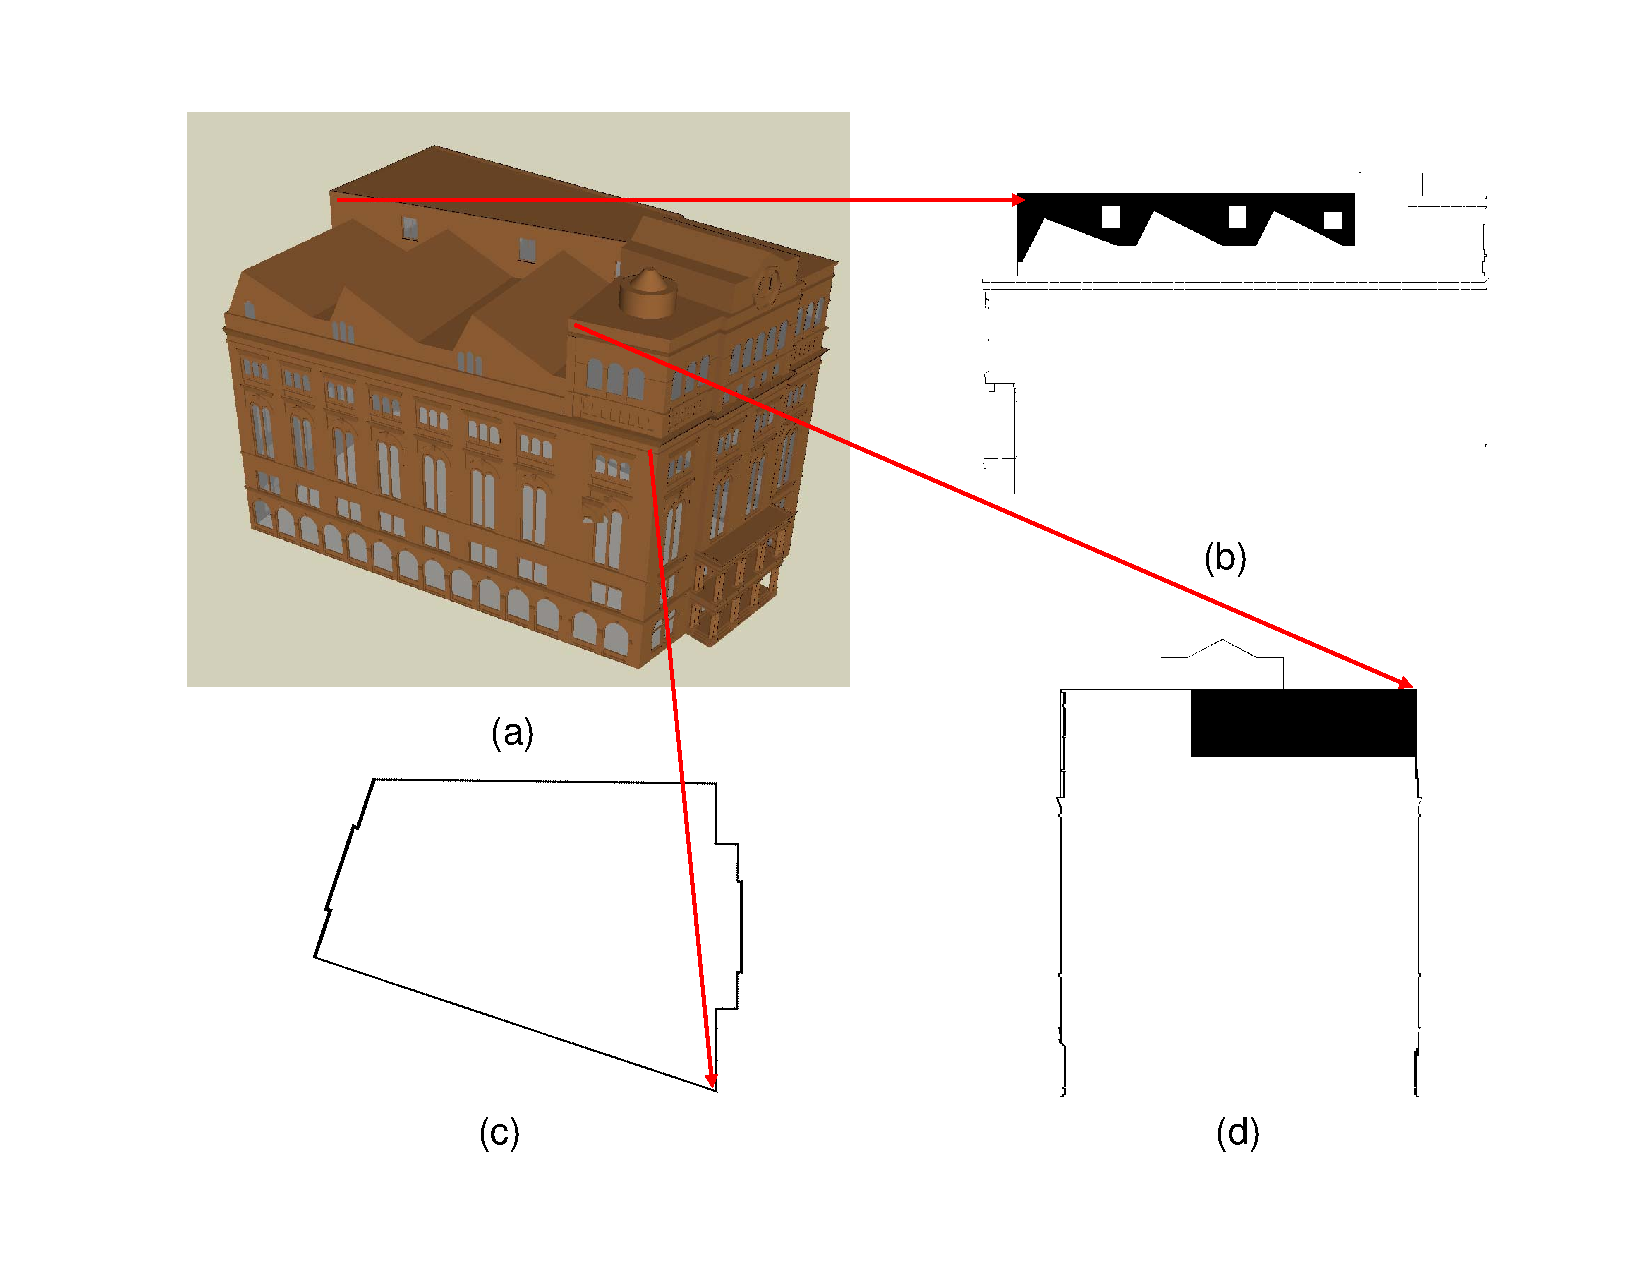
\includegraphics
      [width=\textwidth]
      {model_separate.pdf}
      \caption{The dataset segmentation: 
      (a) the original cooper union model.
      (b) the projected wall image from one face.
      (c) the projected ledger image.
      (d) the projected wall image from another face.}
      \label{fig:MS_Fig1}
\end{figure}

The dataset segmentation is carried out as follows.
First, for a given point cloud dataset, 
we compute separators from all major directions obtained earlier, 
including bottom-up direction and directions perpendicular to major planes.
The next step is to split the original 3D dataset into segments 
based on the computed separators together with direction information.
We will elaborate these steps in the following sections.

\subsection{Separator Detection}
\label{sec:sd}

We used a kernel based connected components (CC) method for computation.
For each identified slice image $I_i$, the separator detector 
checks each data point $P_i$ using a $5$x$5$ kernel $K$ centered at $P_i$.
Let $S_p$ be a set of points that have been visited by the separator detector.
$S_p$ is initialized to be empty.
The point $P_i$ is checked against $S_p$ to 
determine whether it has been visited previously. 
If not, $P_i$ is added into $S_p$ and 
the data points $N=\{P_j | P_j \neq P_i, P_j \in K\}$ 
covered by the kernel $K$ are recorded.
If there are enough data points found in the neighbor, 
say $|N| > 12$, namely half of the kernel $K$, 
$P_i$ is considered as qualified point for the connected component
and is added to $C$. 
The same computation is applied to all new recorded data point in $N$, 
and qualified points are added into $C$. 
When there is no more new data point needs to be checked, the detector stops
and a new connected component, $C$, is detected.

The next step is to compute the rectangle boundary of $C$,
$\{x_{min}$, $x_{max}$, $y_{min}$, $y_{max}\}$.
To check whether $C$ represents a qualified separator, 
the following test is conducted,
\begin{equation*}
\left\{
\begin{array}{lr}
| x_{max} - x_{min} | > T_{size} \\
| y_{max} - y_{min} | > T_{size}
\end{array} \right.
\end{equation*}
where $T_{size}$ is a threshold representing the minimum size of the separator, 
usually a value of $16$ is good enough to rule out all non-separators.
The above testing implies that a real separator CC 
should contain a big chunk of data 
and its width and height should be at least $T_{size}$. 
If a connected component $C$ satisfies the above conditions, 
the slice index $i$ together with the bounding information 
$x_{min}, x_{max}, y_{min}, y_{max}$, 
are logged down for further process.

\begin{figure}[htbp]
\begin{center}
\begin{tabular}{c}
\fbox{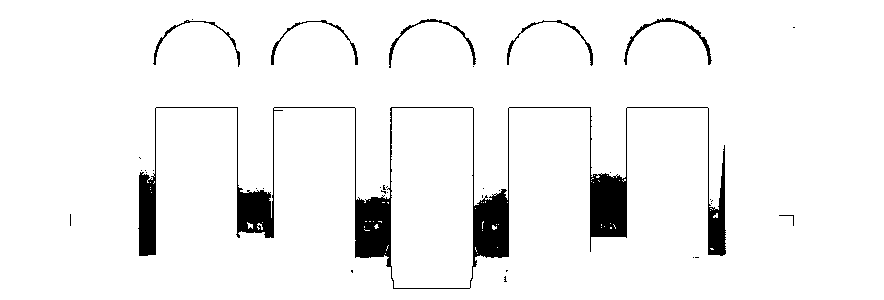
\includegraphics[width=0.7\textwidth]{segment_slice_0254.png}} \\
(a) \\
\fbox{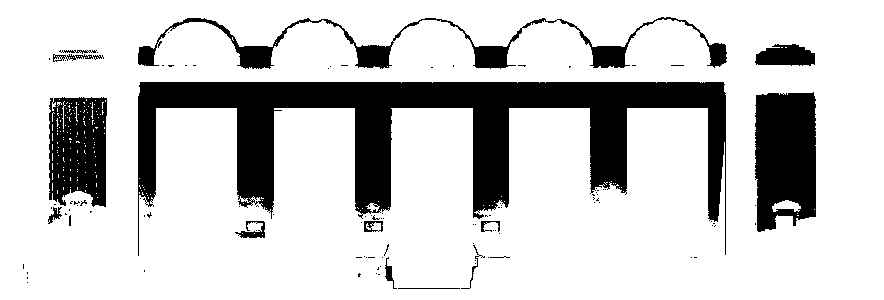
\includegraphics[width=0.7\textwidth]{segment_slice_0255.png}} \\
(b) \\
\fbox{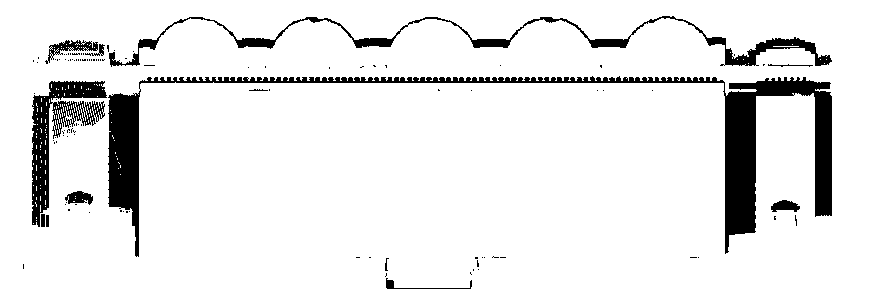
\includegraphics[width=0.7\textwidth]{segment_slice_0256.png}} \\
(c) \\
\fbox{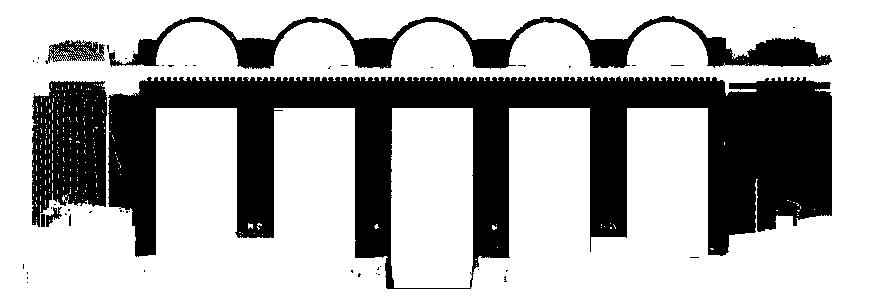
\includegraphics[width=0.7\textwidth]{segment_merged_slice.png}} \\
(d) \\
\end{tabular}
\end{center}
\caption{The adjacent slices with separators detected.
(a) the first slice.
(b) the second consecutive slice.
(c) the third consecutive slice.
(d) the merged slice from (a) to (c).
}
\label{fig:segment_merged}
\end{figure}

For real dataset, separators might be detected in adjacent or 
neighboring sliced images as shown in \Fig{segment_merged} (a) - (c).
This is usually caused by imperfect major plane detection 
or point cloud data registration introduced in earlier stages.
To cope with this case automatically, 
we integrate all the neighboring sliced images 
with separators detected into a new image $I$ as shown in \Figd{segment_merged}.
And the same separator detection algorithm is applied on $I$
to obtain the bounding information.
The index for this integrated image is set to be the mean
of the indices of those neighboring images.
After this automatic computation, we present the results to users
and allow them to adjust the results manually.
Essentially, users can adjust the index of the integrated image, 
which could avoid any potential errors for segmentation.

\subsection{Segmentation Based on Separators}

%%% TWO PARTS:
%%% 1. segmentation on 2D slices.
%%% 2. demonstration on 3D PCD.

%%% show (c) and (d) for 3D PCD segmentation.
%%% show (a), (b) and their superimpose images as 2D slice segmentation.
%%% for 2D sliced image segementation, show a superimposed image and its
%%% segmented region with each region shown as a small image in PPT.

Once we have computed the separators from the salient features, 
such as ledgers or walls, from the sliced images,
we can divide the original complex building structures into
smaller and simpler modules for modeling.
Based on the type of the input data we are about to segment,
two approaches could be adopted for this partitioning process.
First, the segmentation can be carried out on 
the original 3D point cloud dataset. 
That is, a series of smaller 3D point cloud datasets will be
generated for each segment.
However, for this approach, we have to transform each
smaller segment and generate the projected 2D images 
for each major facades.
This would impose redundant projection
and the noise removal and hole filling would have to be applied again.
Alternatively, we can apply the segmentation directly on 
the 2D sliced images generated previously,
and therefore avoid those redundant transformation 
and projection computation required for the first approach.

\begin{figure} [htbp]
\begin{center}
\begin{tabular}{cc}
\fbox{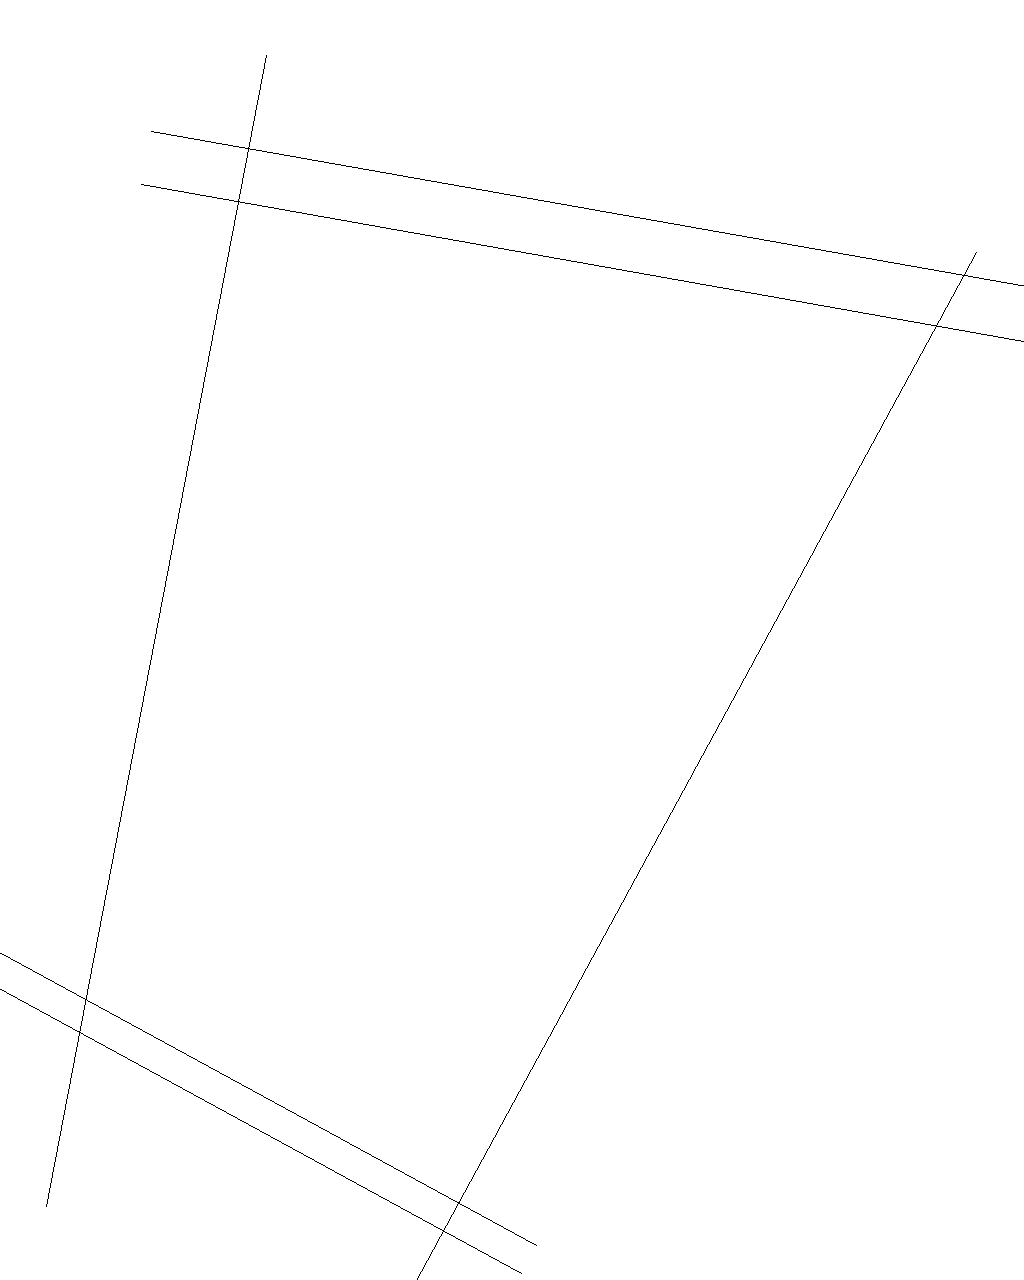
\includegraphics[width=0.4\textwidth]{segment_body_result.png}} &
\fbox{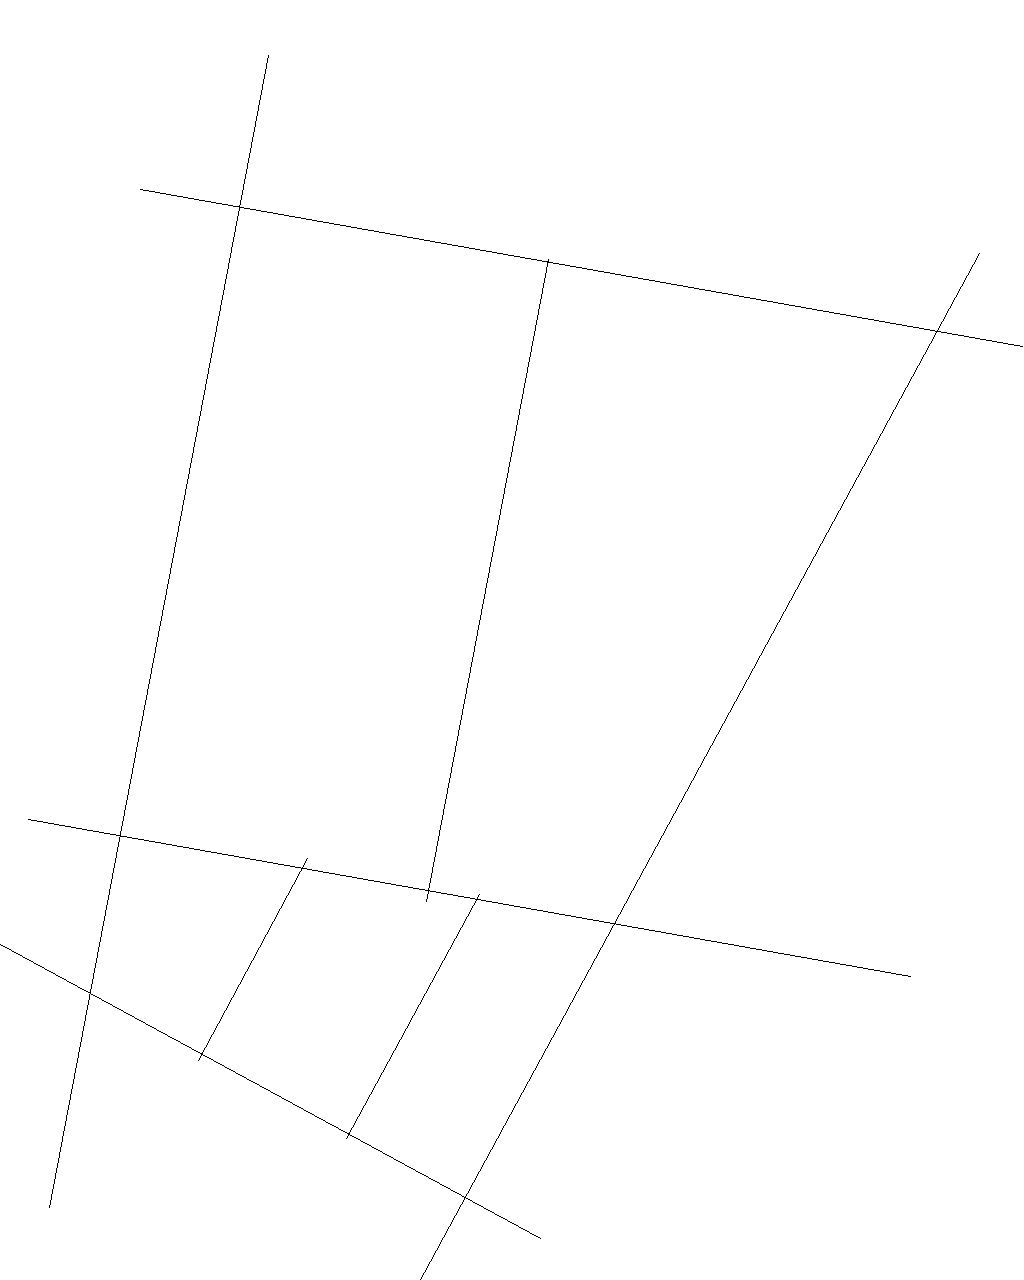
\includegraphics[width=0.4\textwidth]{segment_roof_result.png}} \\
(a) & (b) \\
\fbox{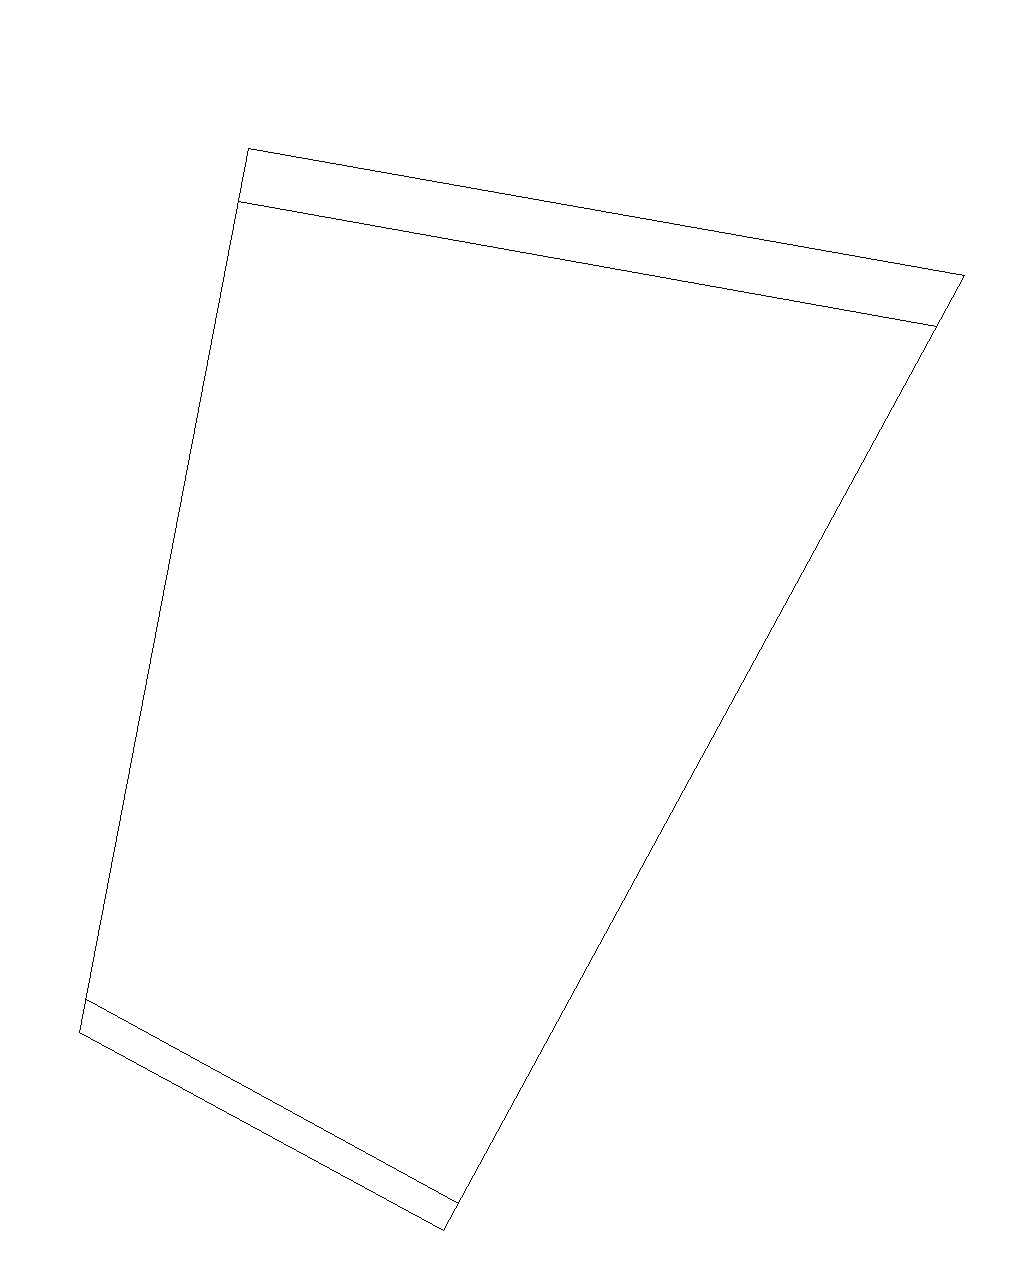
\includegraphics[width=0.4\textwidth]{segment_body_result_region.png}} &
\fbox{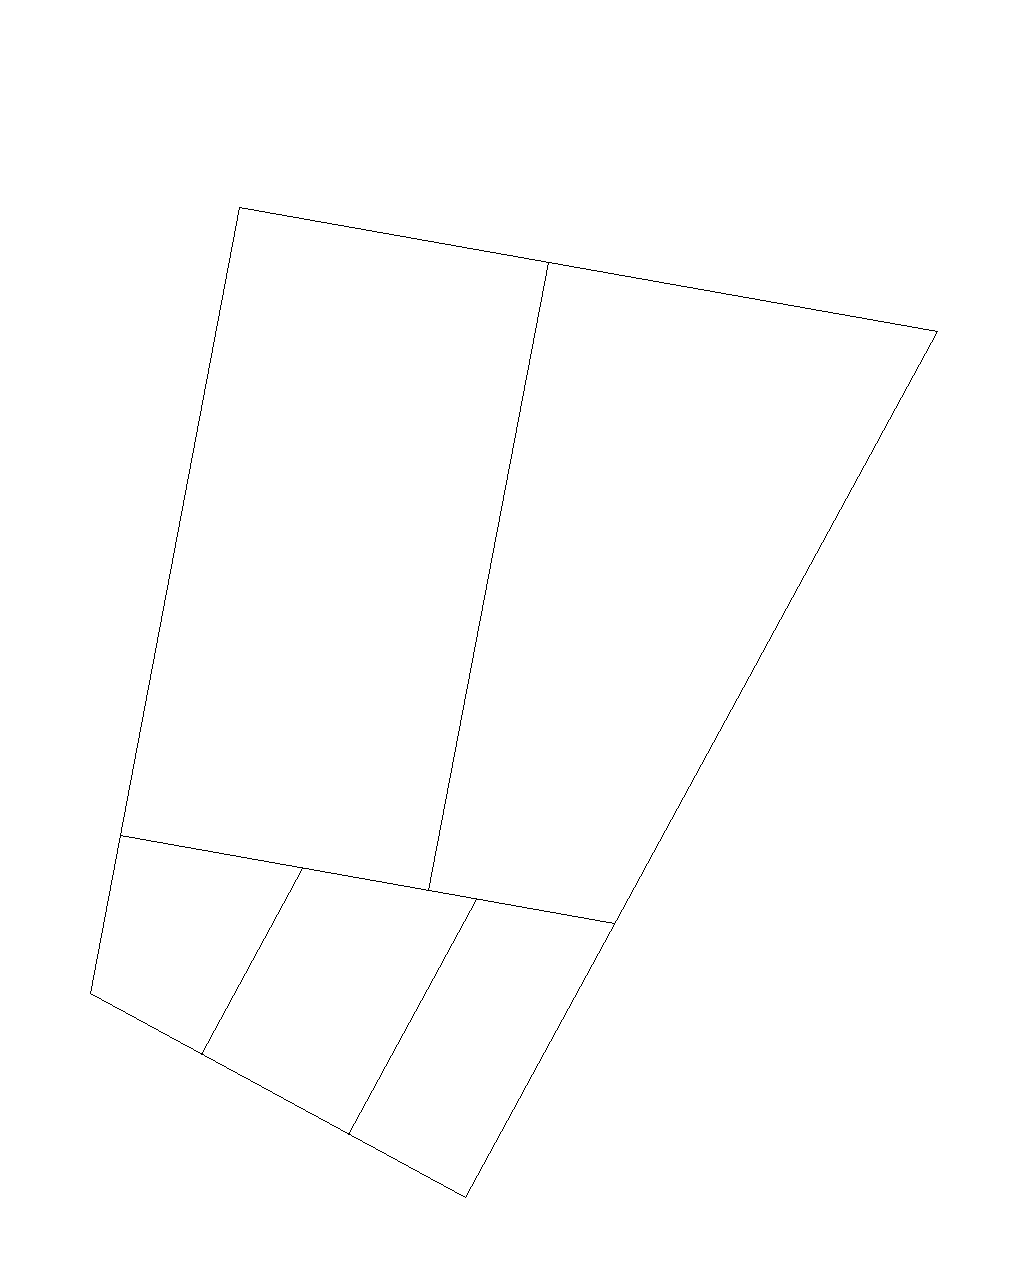
\includegraphics[width=0.4\textwidth]{segment_roof_result_region.png}} \\
(c) & (d) 
\end{tabular}
\end{center}
\caption{ Segmentation region computation:
      (a) the transformed image with line segment of the separators for body,
      (b) the transformed image with line segment of the separators for roof,
      (c) the processed segment image regions for body,
      (d) the processed segment image regions for roof. }
\label{fig:DS_Fig1}
\end{figure}

\begin{figure} [htbp]
\begin{center}
\begin{tabular}{cc}
\fbox{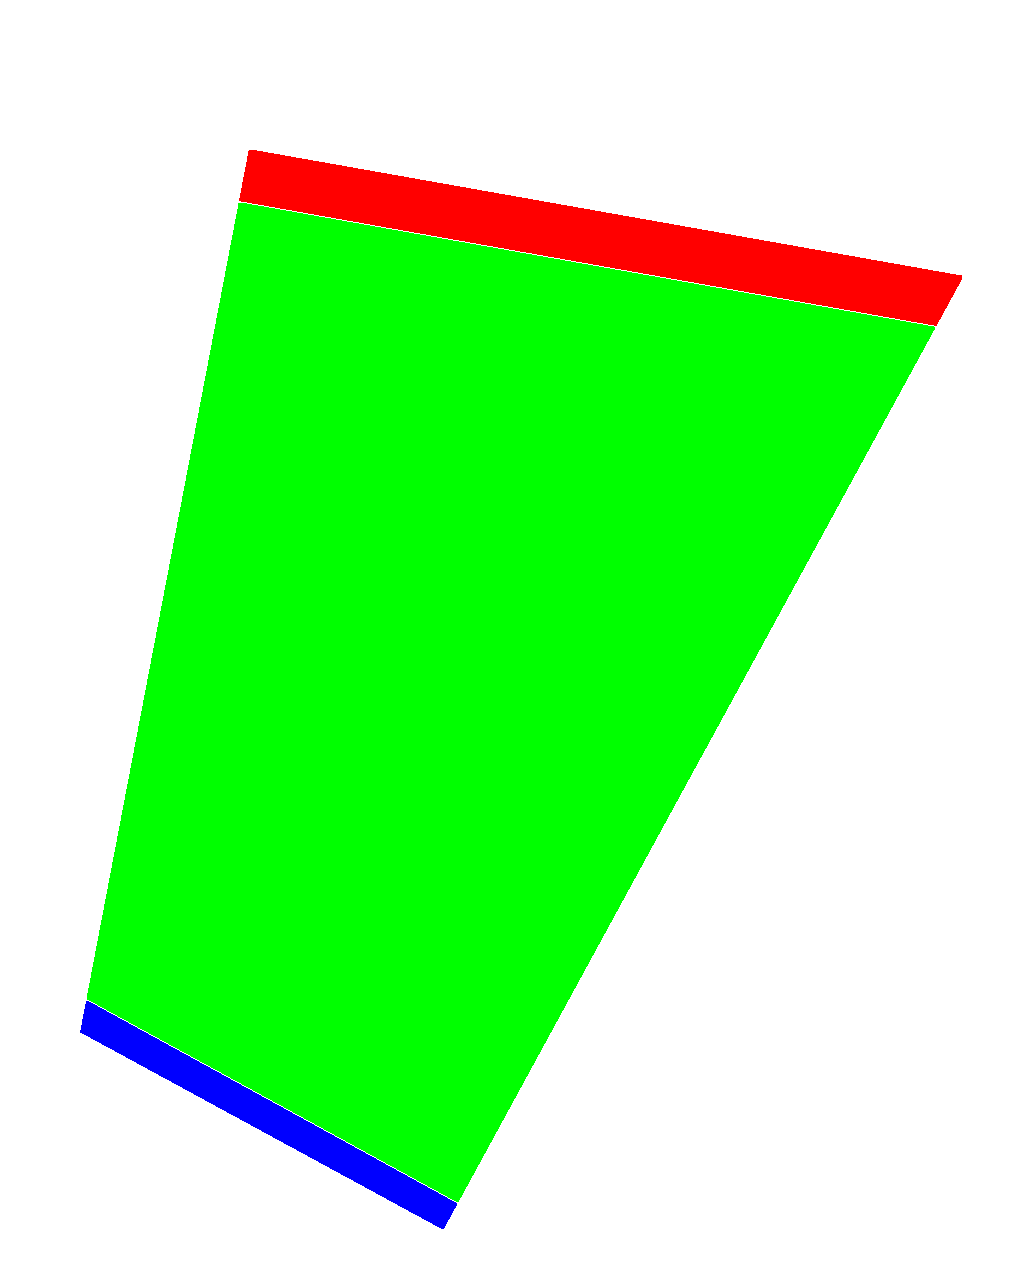
\includegraphics[width=0.4\textwidth]{segment_body_regions.png}} &
\fbox{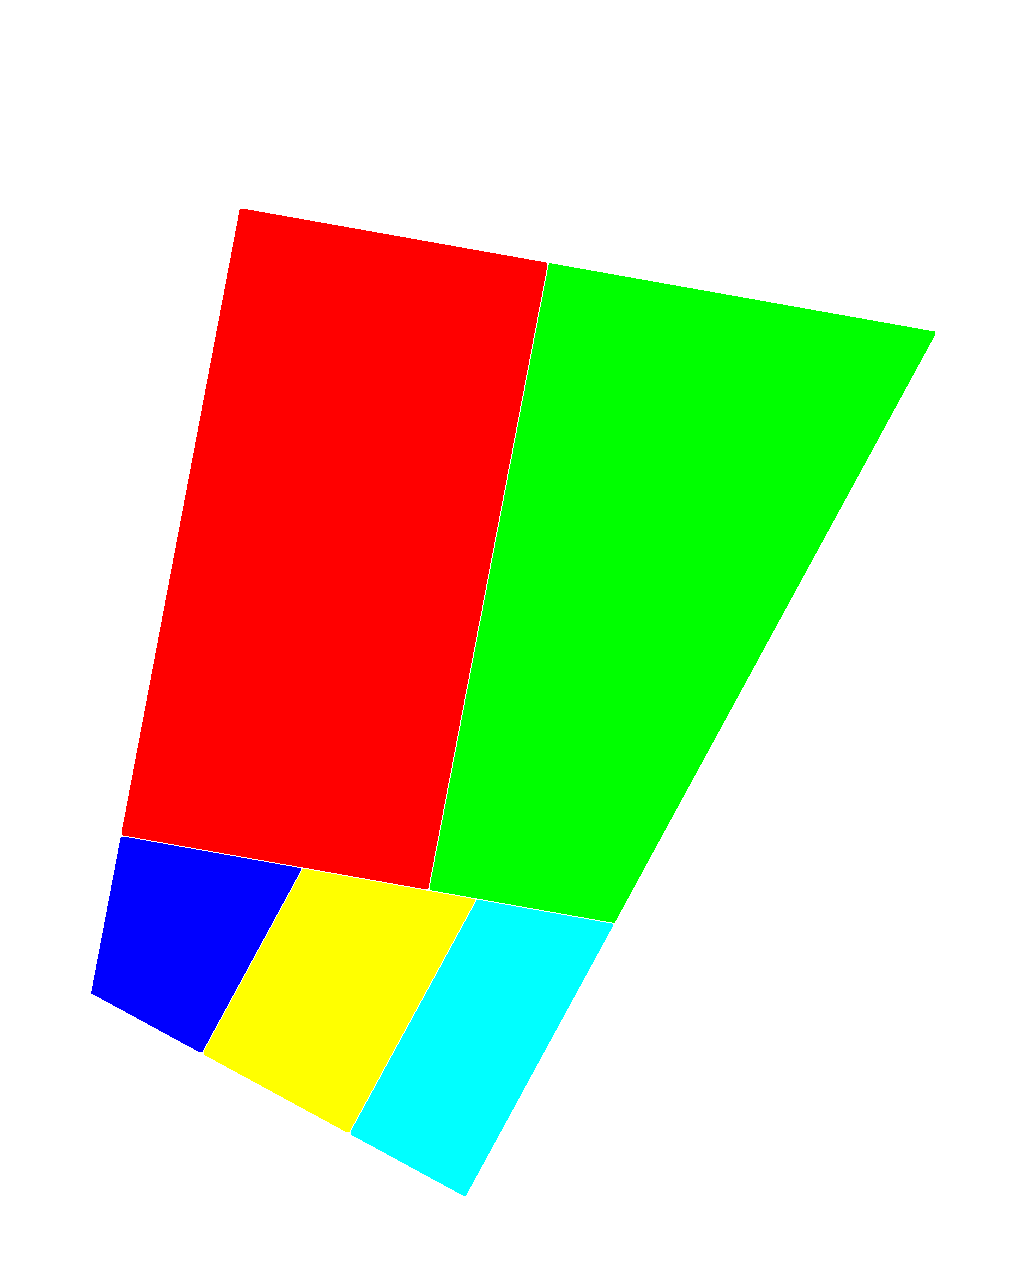
\includegraphics[width=0.4\textwidth]{segment_roof_regions.png}} \\
(a) & (b) \\
\fbox{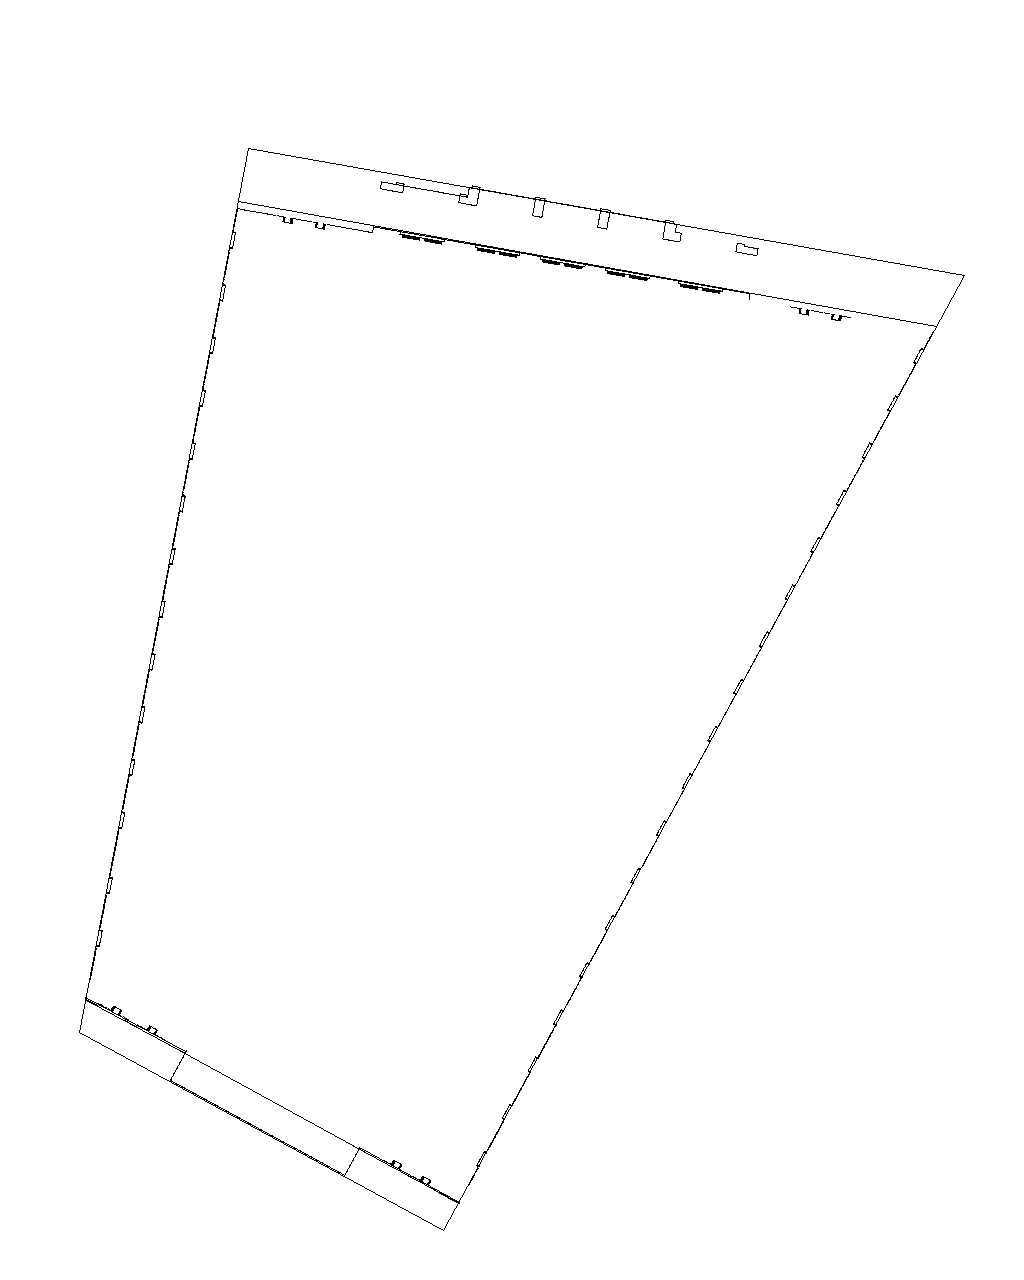
\includegraphics[width=0.4\textwidth]{integrate_body.png}} &
\fbox{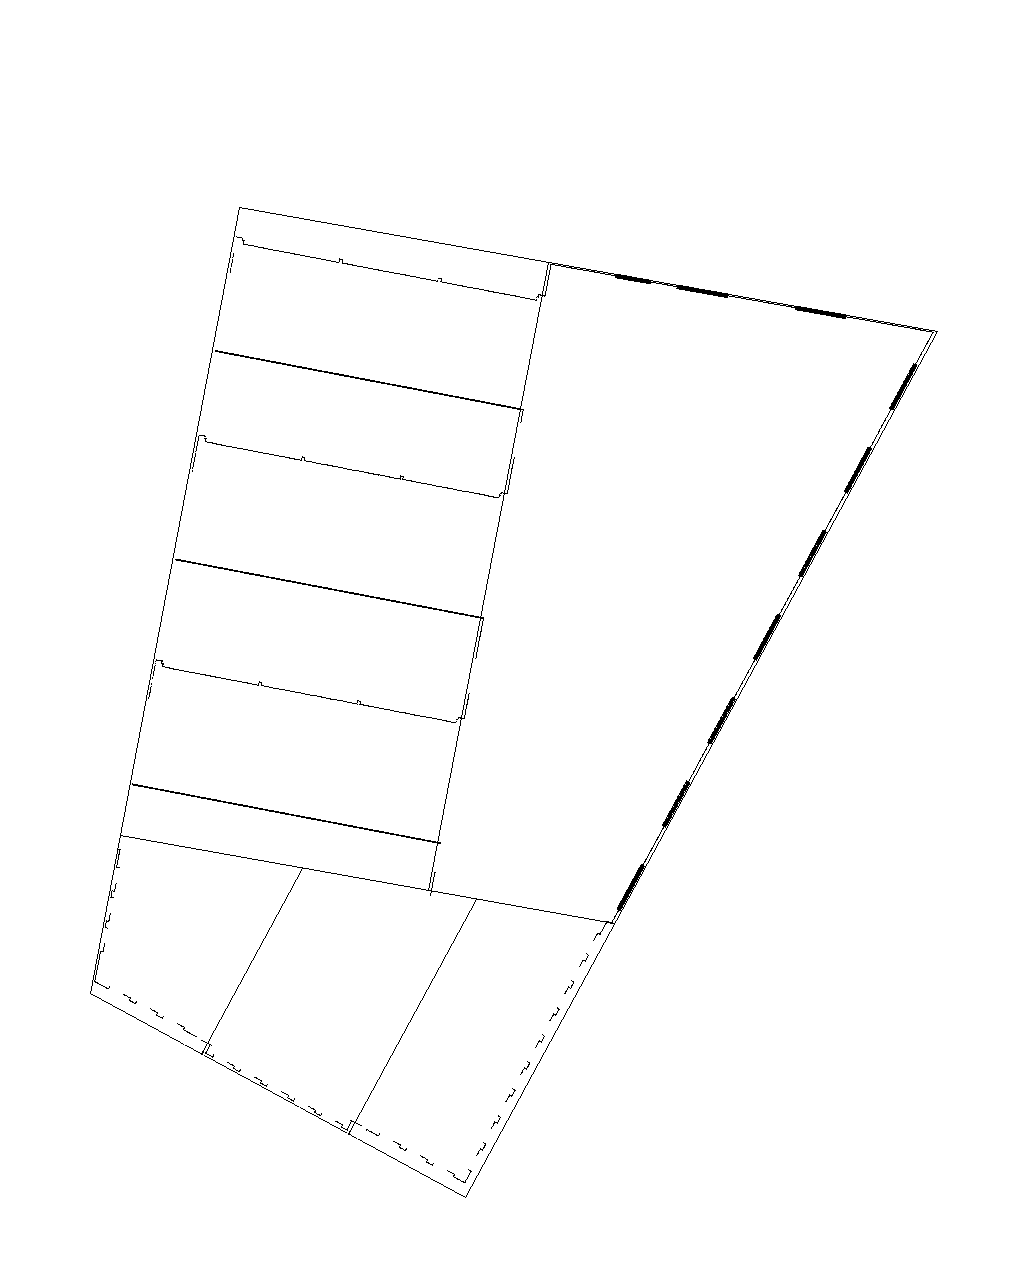
\includegraphics[width=0.4\textwidth]{integrate_roof.png}} \\
(c) & (d) 
\end{tabular}
\end{center}
\caption{ Segmentation region computation:
      (a) the highlighted regions for \Figc{DS_Fig1},
      (b) the highlighted regions for \Figd{DS_Fig1},
      (c) the superimposed image of \Figc{DS_Fig1} with a sliced image from body section,
      (d) the superimposed image of \Figd{DS_Fig1} with a sliced image from roof section.}
\label{fig:DS_Fig1_1}
\end{figure}


% xxx -- backup
%However, manipulating the segmentation on sliced images
%also put the constraint on the segmented smaller images because
%we do not have the control on the size and resolution 
%which have been fixed on the input 2D sliced images.
%We have tried both approaches, and found that 
%the first approach does not slow down much but does offer
%greater flexibility on the manipulation of the segments.
%The second approach also works well on the segmentation.
%So either method is ok.

%% bottom-up division
To conduct the segmentation for the 2D sliced images,
we need to transform the separators in all directions 
into the common coordinate (with $y$-axis as the bottom-up direction).
Because the separators detected in bottom-up direction
are already in the common coordinate,
no transformation is needed for these separators
and the partitioning is straight-forward:
%
we first sort the indices $I$ of the bottom-up separators 
in an ascending order.
The 2D slices projected along bottom-up directions
are grouped based on their indices against the sorted indices $I$.
For example, a group of the range from $I_i$ and $I_{i+1}$,
contains all 2D slices with index between $I_i$ and index $I_{i+1}$.
%
For the example in \Figa{syn_data},
The only detected separator (the ledger) as shown in \Figc{MS_Fig1}
divides the whole dataset into top (roof structure) and
bottom (body structure).

%% other directions
The process becomes harder when we start the segmentation 
on the 2D slices in the same group of height section.
First of all, all the separators detected in different directions
need to be brought to the common coordinate.
Each separator is transformed into 
a line segment in the bottom-up projected image with the end points 
representing the bounding positions.
The roof and body projected images are shown in 
\Figa{DS_Fig1} and \Figb{DS_Fig1} respectively.
To compute the boundary for each segment,
the intersection points 
for each line segment with other line segments need to be computed.
%
Given a line segment $L_i = P_0P_1$, represented by two end points $P_0$, $P_1$, 
we can compute the intersection points of
$L_i$ with all other line segments. 
%[ with the equation of intersection computation of two planar lines].
If the result intersection point $P_i$ is falling outside of the image or 
is far away from either $P_0$ or $P_1$, 
$P_i$ is an intersection point that is not belong to the building,
and therefore it can be skipped.
When all the other line segments are checked, 
we can obtain two special intersection points, $P'_0$ and $P'_1$, 
which are the closest ones to $P_0$ or $P_1$ respectively. 
$P'_0$ and $P'_1$ represent the starting and ending points
for the walls or features of the building.
After intersection points are computed for all line segments, 
the segmentation image $I_s$ can be obtained.
\Figc{DS_Fig1} and \Figd{DS_Fig1} illustrate the computed segmentation images
for both body and roof sections.

With the segmentation images $I_s$, 
we can compute each segment region for 2D slices projected in bottom-up direction.
To do this, we first build up a look-up table $T$ 
which maps a pixel point $(x, y)$ in $I_s$ to a region,
as shown in \Figa{DS_Fig1_1} and \Figb{DS_Fig1_1} for both body and roof. 
Different regions are marked in different colors 
and are assigned a unique region id. 
For a given point $P(x, y)$ in each sliced images, 
the region id for $P$ can be obtained from the look-up table $T$.
For example, for the roof sliced images,
all red pixels are mapped to the same region id in \Figb{DS_Fig1_1}. 
The same situation is applied to green, blue, and other pixels.
After going through each point, a 2D sliced image from bottom-up direction
can be divided into segments. 
The 2D sliced images for body and roof
with segmentation regions superimposed 
are shown in \Figc{DS_Fig1_1} and \Figd{DS_Fig1_1}, respectively.
%%% segments on major planes other than bottom-up direction
%%%
For those 2D slices projected from normals of other major planes,
we carry out similar strategy for segmentation as that of bottom-up direction.



%% demonstration on 3D PCD
%% show the 3D image
To demonstrate the segmentation results on 3D dataset,
a similar process as 2D sliced image segmentation can be conducted.
For each 3D data point ${\bf P}(x, y, z)$, 
we first compute its group in bottom-up direction
by comparing ${\bf P}$'s $y$ value (bottom-up direction) and 
those heights from range indices.
%
Once the group is computed, with the segmentation image $I_s$, 
we can further compute the region id for ${\bf P}$ by
obtaining its 2D projection point $P(x, y)$ in the image $I_s$. 
%[ based on the equation [equation of the projection].
The region id for $P$ can be obtained from the look-up table $T$.
For the example in \Figa{syn_data},
there are totally 5 regions are identified for data points of roof
and 3 regions are located for body.
Hence the original point cloud of the building is 
segmented into 8 segments as shown in \Fig{DS_Fig2},
where different segments are labeled with different colors.

\begin{figure} [htbp]
\begin{center}
\begin{tabular}{c}
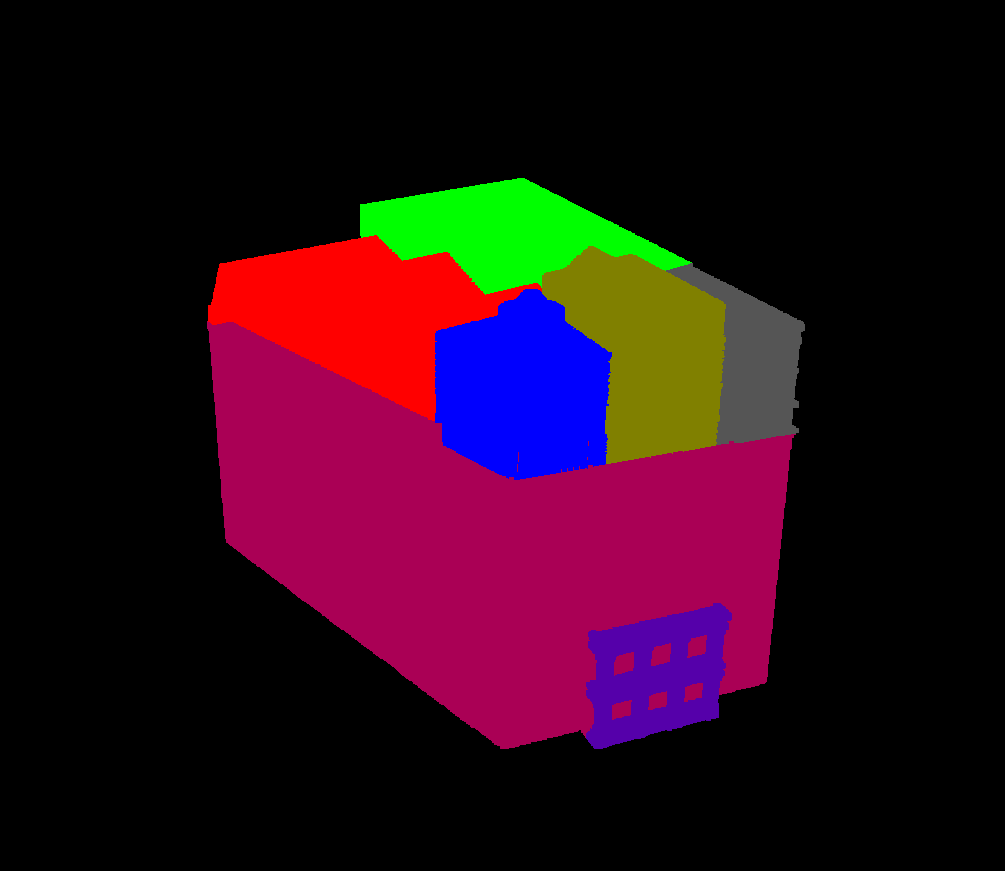
\includegraphics[width=0.75\textwidth]{cu_7.png} 
\end{tabular}
\end{center}
\caption{ the segmentation result for the whole PCD of \Fig{MS_Fig1}.}
\label{fig:DS_Fig2}
\end{figure}


%%%%% New Chapter %%%%%
%%%%% New Chapter %%%%%
\newchapt{Keyslice Detection}{chapt_key}{Keyslice Detection}

\label{sec:reconst}
Our 3D modeling algorithm is based on \emph{a priori} knowledge that
urban buildings can be created through a series of extrusion and tapering
operations on the salient cross-sections contained in the keyslices.
The key step for successful modeling is identifying these salient cross
sections upon which the extrusion and tapering operations will apply.

Buildings generally are equipped with windows and doors which should not
be considered as salient feature for keyslices. 
Therefore, as an necessary preprocessing, 
data points corresponding to windows and doors
should be ruled out to avoid possible side-effects
during the keyslice computation.

\section{Window Detection}
\label{sec:wdd}

Windows and doors are important features for buildings to be modeled. 
Moreover, accurate computation of the extrusion structures 
depends on these information.
Without knowing the marked location as window part, 
extra keyslices may be computed and hence lead to excessive extrusion operations. 
Image-based window detection has been widely conducted in 
\cite{WDD_LN,WDD_TKKJ}.
Essentially, the 2D window regions are extracted by exploiting the properties
of building structures, such as shape and symmetry. 
The estimation of the depth for the extracted 2D windows is computed 
by using matches for the linear features within the extracted
window in two or more ground views.
However, the estimation is not reliable due to perspective projection.
Some window detection methods on 3D data have also been proposed in
\cite{WDD_SV,WDD_BBH}.
A constrained surface fitting and a genetic algorithm 
is proposed to fit parametric models of doors on point cloud in \cite{WDD_FF}.
This method assumes that the data have been segmented 
and requires relatively high density data around the window area.
Pu and Vosselman use a triangulation-based method 
to detect the boundaries of sparse regions within a building facade 
and then fit rectangles to the resulting region to compute windows \cite{WDD_PV}.
However, this method needs to improve its accuracy when background noise exists.

\begin{figure}[htbp]
  \centering
  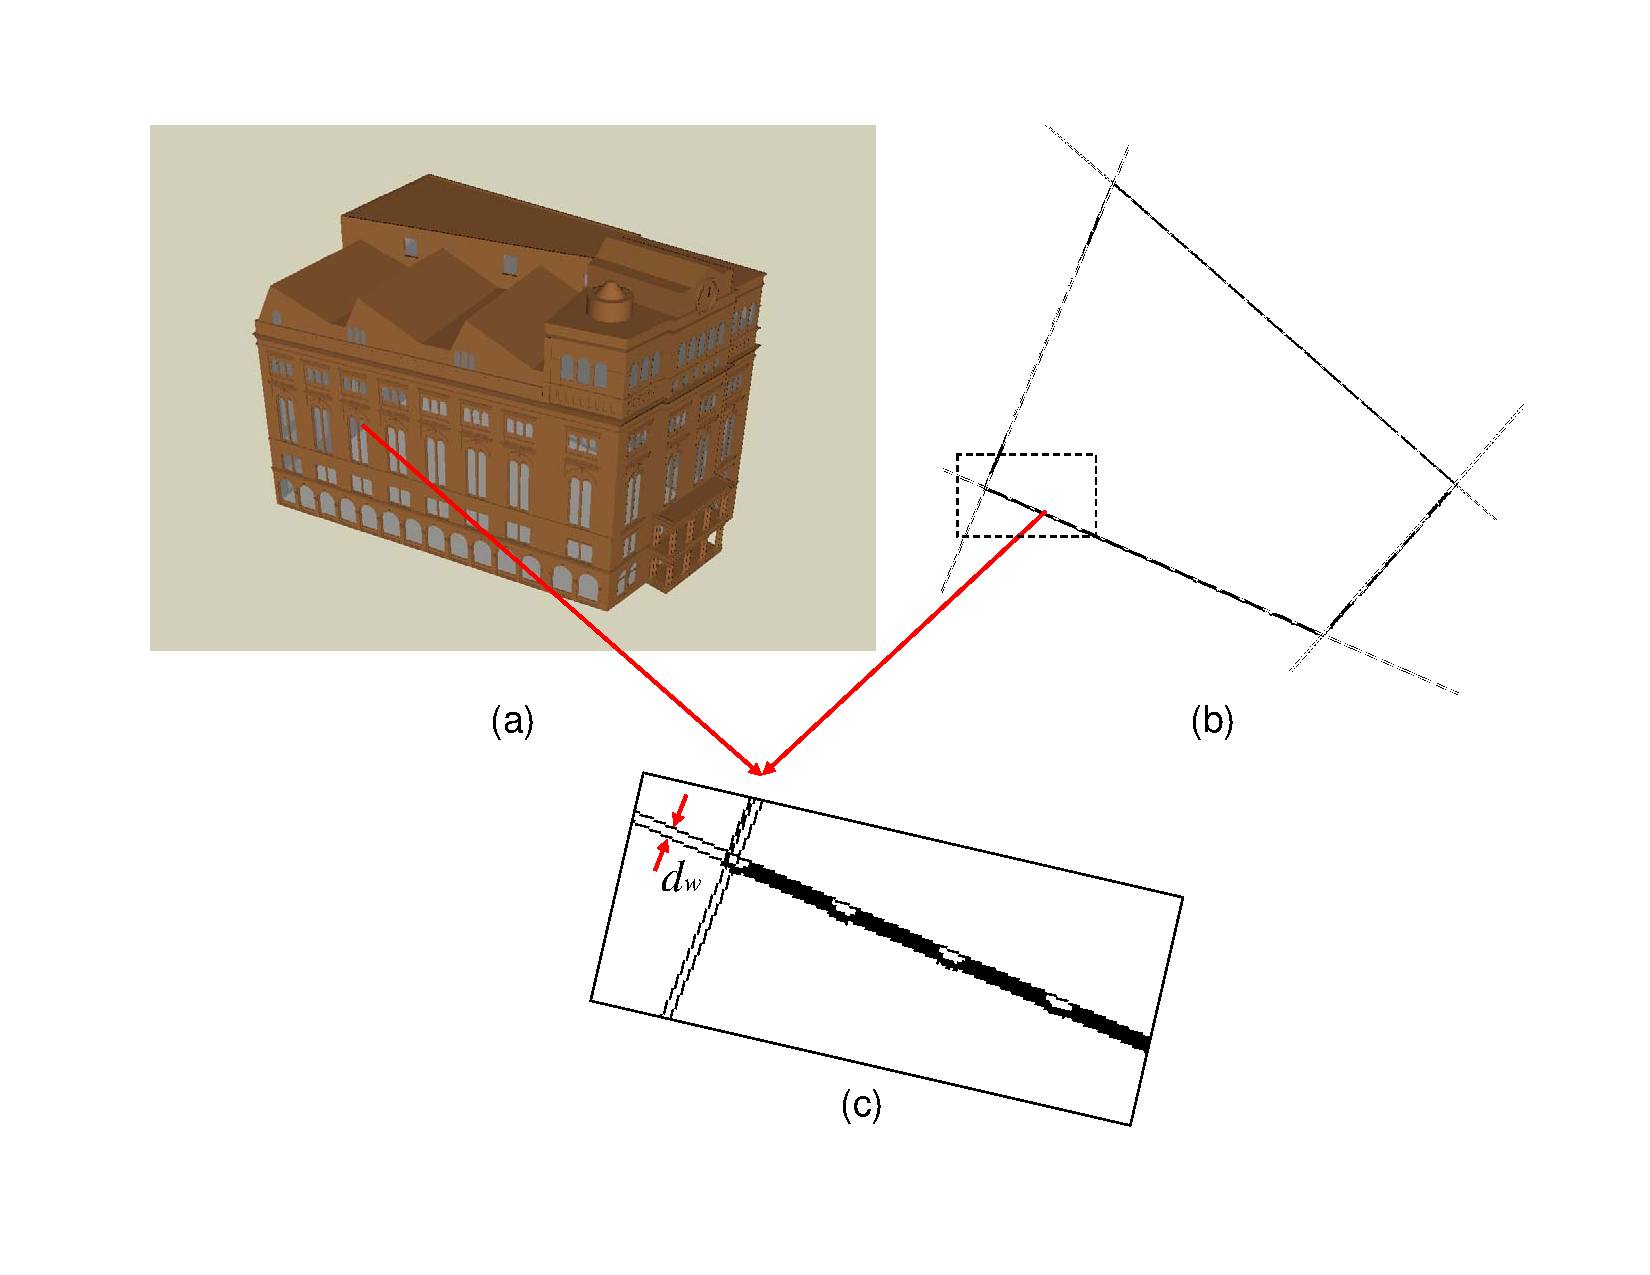
\includegraphics
      [width=\textwidth]
      {model_win_comp.pdf}
      \caption{The thickness detection of the windows/doors:
      (a) the window on the original model
      (b) the projected slice viewing from bottom-up direction
      (c) the close-up view of the parallel lines and the distance $d_w$. }
      \label{fig:WD_Fig1}
\end{figure}

%[show a figure with unnecessary keyslice? how?]
The information we want to compute for windows and doors includes 
both the location and the depth.
The depth is computed based on the observation that two parallel lines can be detected
when viewing from the bottom-up direction as shown in \Figc{WD_Fig1} . 
For two parallel lines $L_1: y = mx + c_1$ and $L_2: y = mx + c_2$, 
% as shown in Fig1, 
% http://www.askiitians.com/iit_jee-Straight_Line/Distance_between_two_parallel_lines
the distance $d_w$ is computed with the following equation,
\begin{equation*}
d_w = \frac{|c_1 - c_2|}{\sqrt{1 + m^2}}
\end{equation*}

%[Fig1: show the window thickness detection image, two parallel lines are drawn]
%[Fig2: show the projected windows/doors slice]

\begin{figure}[htbp]
  \centering
  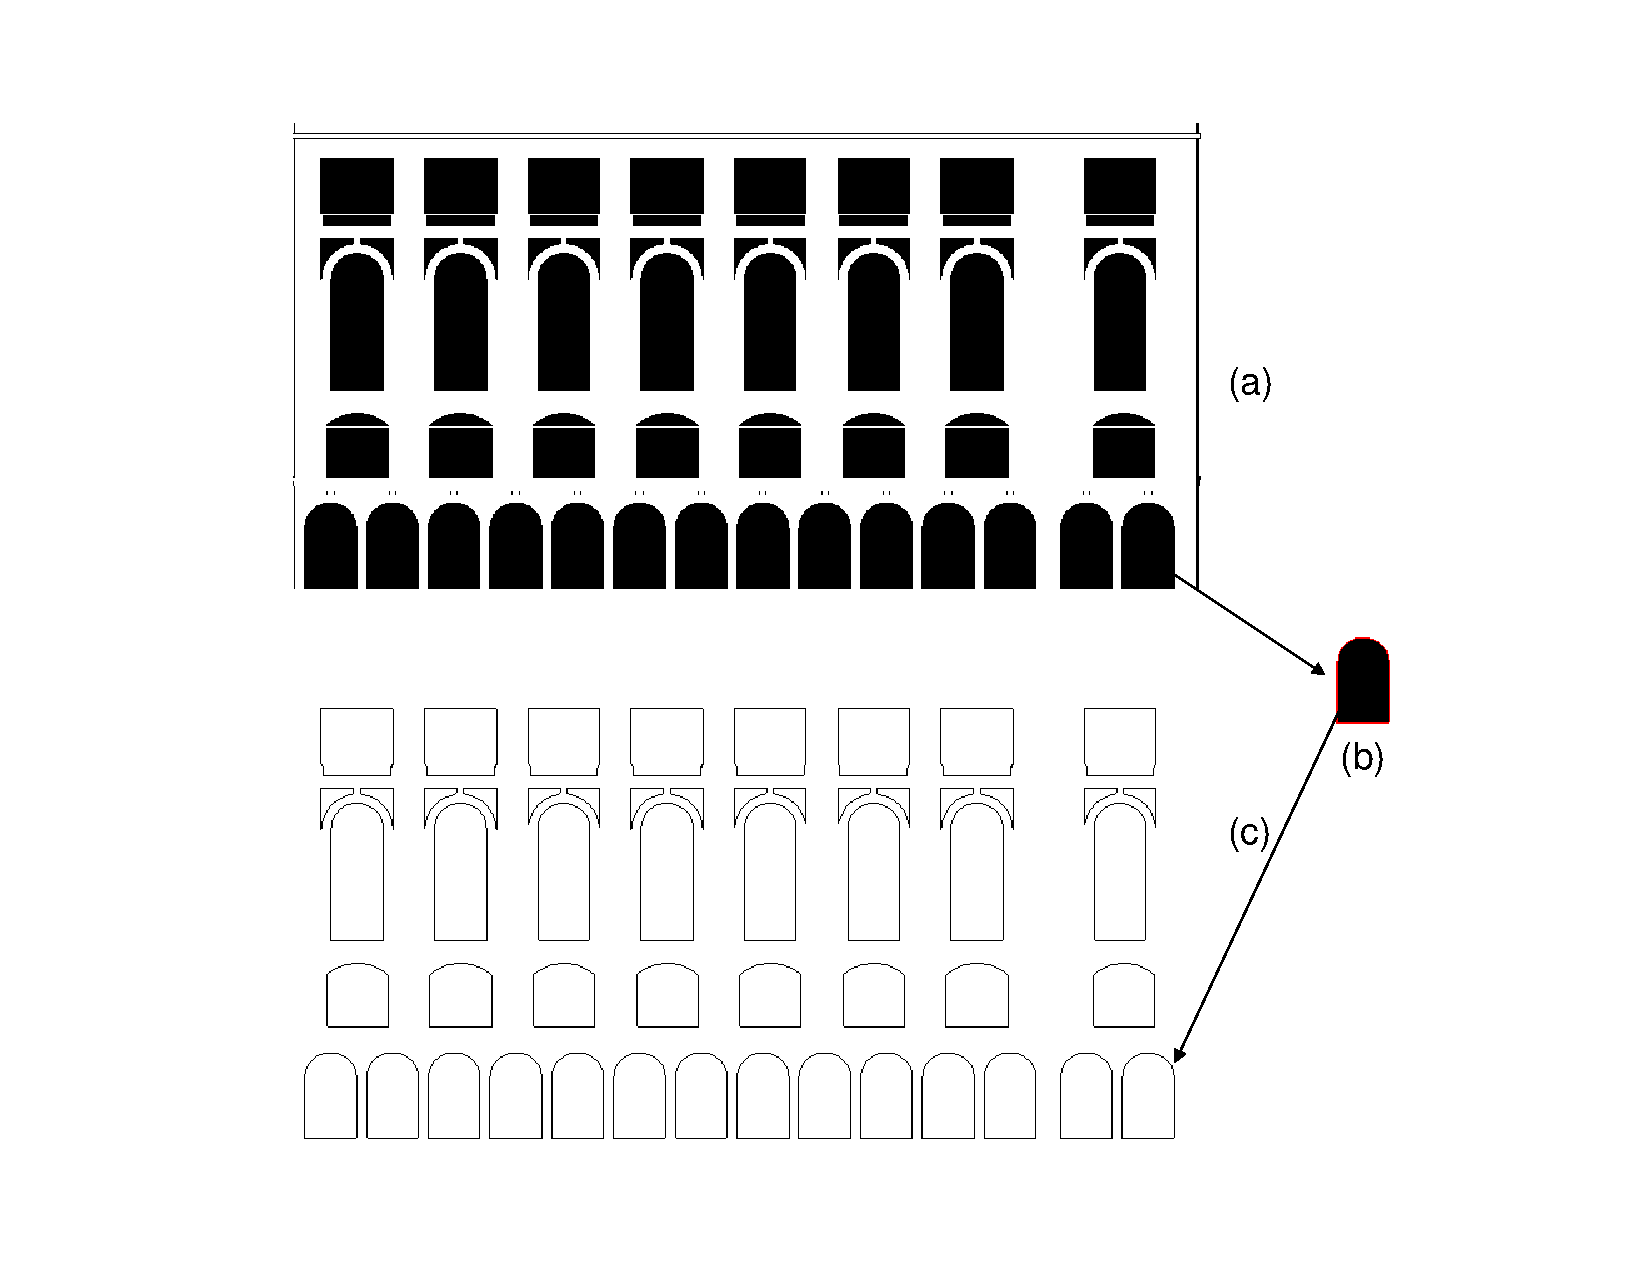
\includegraphics
      [width=\textwidth]
      {window_result.pdf}
      \caption{The window information: (a)The projected windows slice
      (b) the most bottom-right window extracted from (a) with BPA contour in red. 
	(c) The contours of windows computed from (a).}
      \label{fig:WD_Fig2}
\end{figure}

%%% xxx -- not clear
Once the distance $d_w$ is computed, 
we can obtain the windows/doors image by projecting the data points
between $L_1$ and $L_2$ onto a slice image as shown in \Figa{WD_Fig2}. 
There are multiple window structures in the same projected slice image. 
We can use the same strategy as separator detection described in \Sec{sd}, that is,
kernel based connected component method, to isolate each window for processing. 
\Figb{WD_Fig2} shows a window extracted as a connected component and BPA algorithm was applied
to obtain the contour in red.
After walking through the image shown in \Figa{WD_Fig2} for all the connected components 
and applying BPA on them, 
the final results show all the detected window contours as depicted in \Figc{WD_Fig2}.
These contours will be used to add windows and doors onto the final model.

The above window detection is for synthetic dataset since clean result can be obtained. 
For real dataset, the window image computed is too complicated to 
be processed using the above method and therefore manual efforts
are needed to assist the computation.
First of all, the user should check whether excessive data points are included
when projecting the data points to generate the window image 
between $L_1$ and $L_2$. For example,
\Fig{WD_Fig3}(a) - (d) show the consecutive projected images with window structures.
As we can see, \Figd{WD_Fig3} also contains walls (the black regions).
\Fig{WD_Fig3}(e) show the integrated image for slices (a) - (c) and
\Fig{WD_Fig3}(f) show the integrated image for slices (a) - (d).
Apparently, \Fig{WD_Fig3}(f) contains excessive data points for window image
and therefore not suitable for window structure computation.
Secondly, some data are missing around the window as shown in \Fig{WD_Fig3}(e).
In this case, we may have to manually enhance the window boundary 
as shown in \Fig{WD_Fig3}(g). 
With the assistance of user interaction, we can obtain the final window 
structure as shown in \Fig{WD_Fig3}(h).

\begin{figure}[htbp]
\begin{center}
\begin{tabular}{ccc}
\fbox{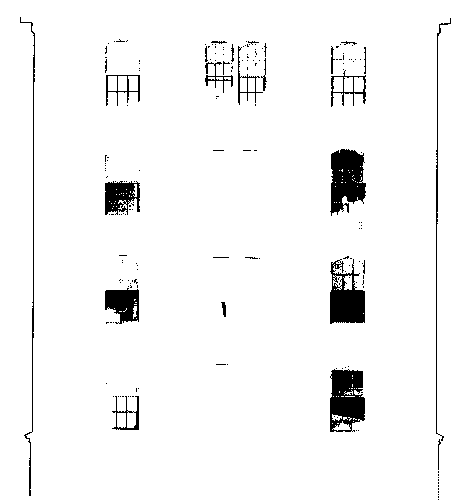
\includegraphics[width=0.3\textwidth]{image_slice_0736.png}} &
\fbox{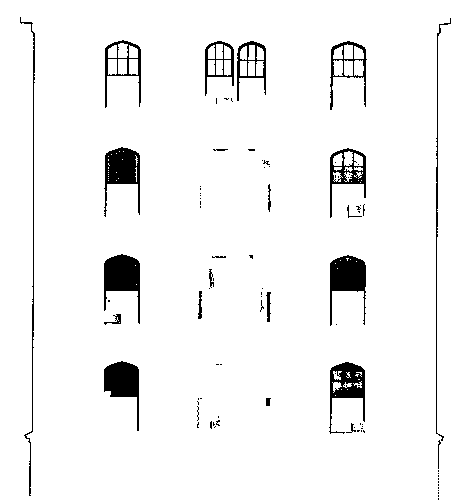
\includegraphics[width=0.3\textwidth]{image_slice_0737.png}} &
\fbox{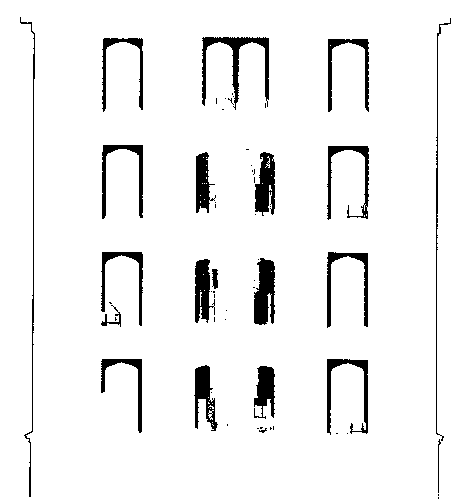
\includegraphics[width=0.3\textwidth]{image_slice_0738.png}} \\
(a) & (b) & (c) \\
\fbox{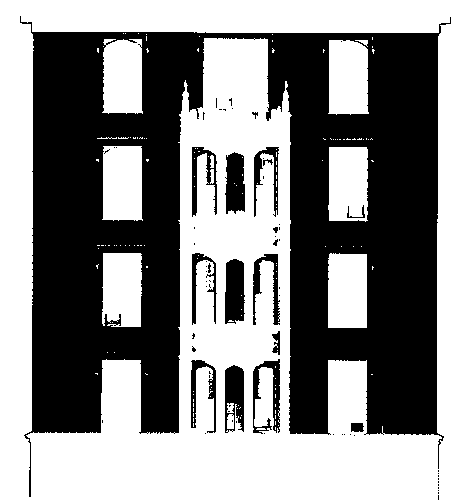
\includegraphics[width=0.3\textwidth]{image_slice_0739.png}} & &
\fbox{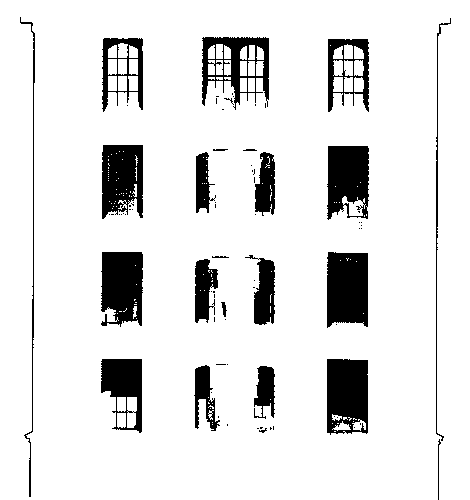
\includegraphics[width=0.3\textwidth]{image_slice_0736_0739.png}} \\
(d) & & (e) \\
\fbox{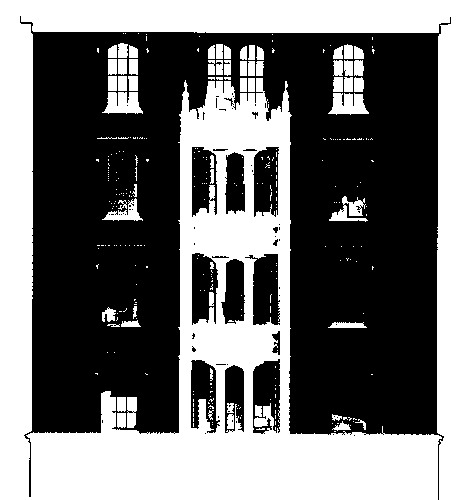
\includegraphics[width=0.3\textwidth]{image_slice_0736_0740.png}} &
\fbox{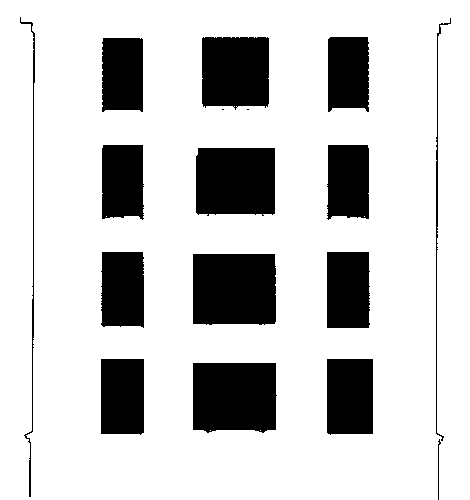
\includegraphics[width=0.3\textwidth]{sym_image_0736_0739.png}} &
\fbox{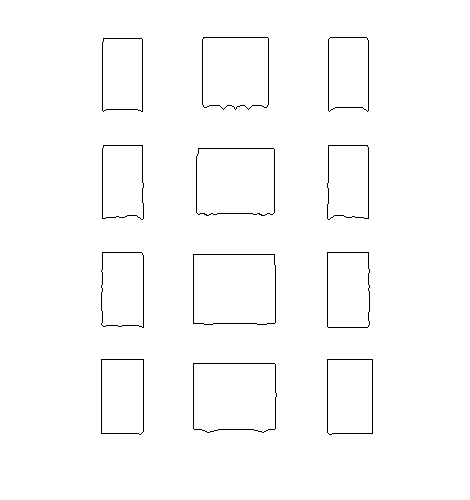
\includegraphics[width=0.3\textwidth]{sym_image_0736_0739_out.png}} \\
(f) & (g) & (h) \\
\end{tabular}
\end{center}
\caption{
Window detection for real dataset. (a) - (d) are consecutive slices. 
(e) integrated slice from (a) to (c);
(f) integrated slice from (a) to (d);
(g) manually enhanced image from (e);
(h) window structure computation from (g).
}
\label{fig:WD_Fig3}
\end{figure}


\section{Windows Mask Image Generation}

Windows and doors detection have been discussed in \Sec{wdd}.
If there is no windows or doors structures detected in the current PCD,
this step is skipped.
However, when windows or doors are detected, 
the data points corresponding to these structures in cross-section images 
should not be taken into account for keyslices computation.
This is to ensure that no keyslices are generated
due to curve or any geometry shapes introduced by windows or doors.

To generate the mask images, the information about windows and doors,
including width, height, depth are needed, which has been computed previously.
Let $\{x_{min}, x_{max}, y_{min}, y_{max}, z_{min}, z_{max}\}$
be the bounding box $w_{box}$ of a window $w$,
where $x, y, z$ are corresponding to width, height and depth directions.
The $w_{box}$ is transformed to bottom-up direction,
with $x, z$ defining the rectangle location of the window,
and with $y$ defining the height range for $w$.

\begin{figure}[htbp]
\begin{center}
\begin{tabular}{cc}
\fbox{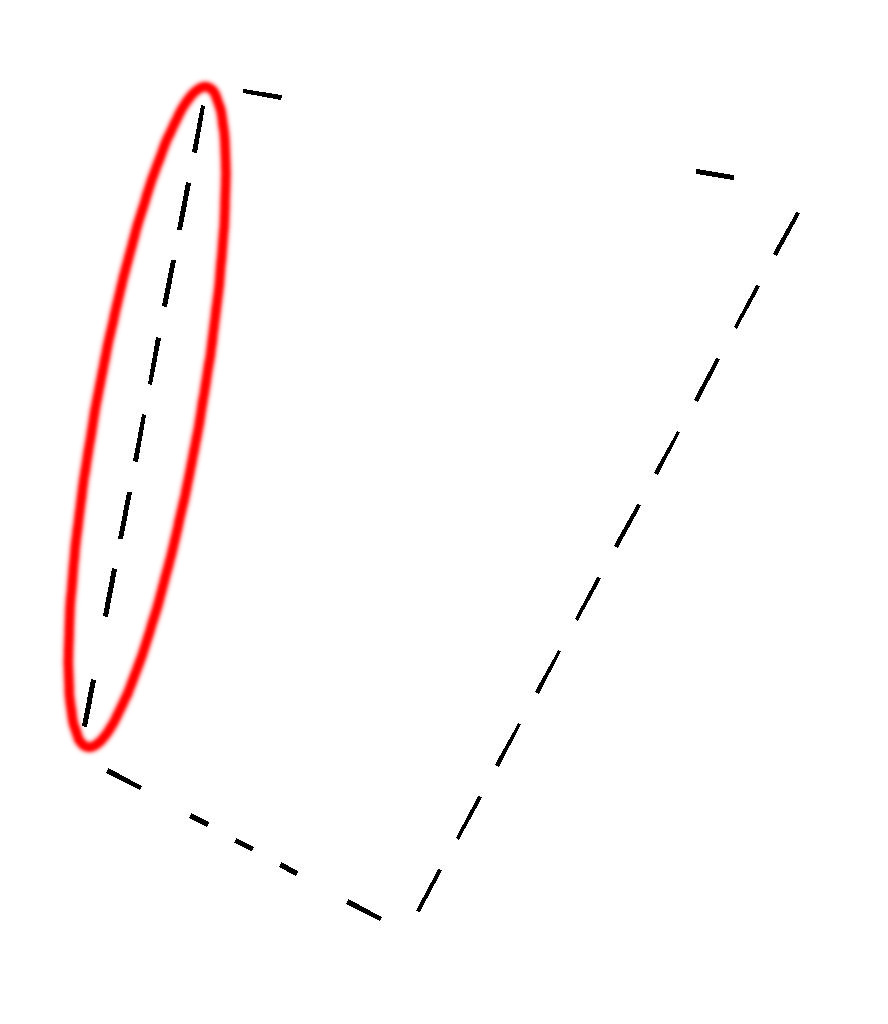
\includegraphics[width=0.4\textwidth]{window_mask_1.jpg}} &
\fbox{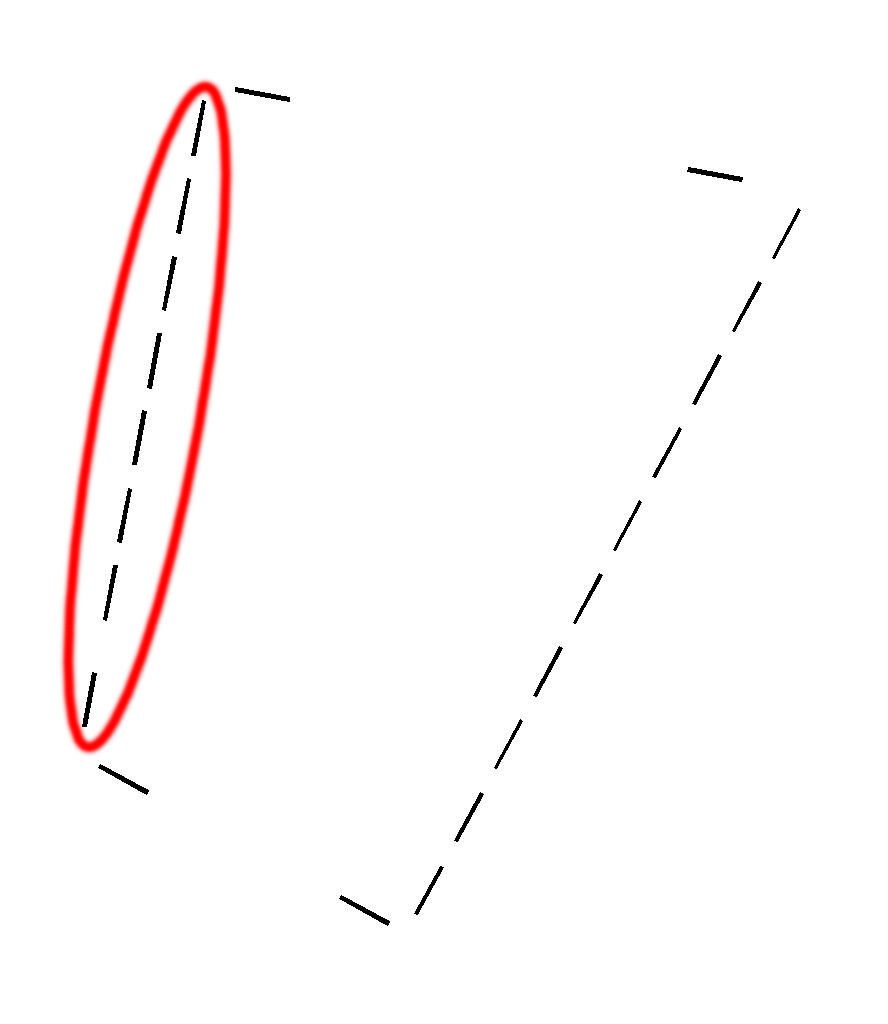
\includegraphics[width=0.4\textwidth]{window_mask_2.jpg}} \\
(a) & (b)
\end{tabular}
\end{center}
\caption{The window mask images: 
         (a) The mask image corresponding to height range of bottom windows.
	 (b) The mask image corresponding to height range of upper windows.}
\label{fig:WD_Fig3}
\end{figure}

After computing the mask information for all windows, 
the mask images can be generated by fusing all the window information. 
\Fig{WD_Fig3} shows couple of mask image examples 
for different height range of the cross-section slices.
The regions circled in red are corresponding to 
the locations of the windows in \Figa{WD_Fig2} in different height range.

Once the mask images are obtained, 
a simple bit-and operation with the original 2D slice image 
eliminates the data points corresponding to windows or doors.
That is, $I_n = I \, \& \, I_w$, where $I$ is a 2D slice, $I_w$ is the mask image,
and $I_n$ is the updated 2D slice with window or door data points removed.
The updated $I_n$ slices are used for keyslice detection.

